% !TeX root = ../main.tex
% Add the above to each chapter to make compiling the PDF easier in some editors.

\chapter{Introduction}\label{chapter:introduction}

It is safe to say that the internet paved the way of many things for humanity.
Media such as images, video and audio can be shared across websites and applications, knowledge can be stored in faraway servers and retrieved with ease in text format using mobile devices, and products and services can be bought with the click of a button or a tap on a screen.
Interactions, media and information make up for massive amounts of data that flow through complex computer systems, which in turn generate even more data and information.

Researchers have found ways to leverage the magnitude of data that is being produced every second by countless systems all around the world.
One of the most recent and most popular uses of this huge variety and quantity of data is machine learning (ML).
Machine learning can be defined as a set of techniques that use data to improve performance in a set of tasks.
Today, for example, we feed data to machine learning models to calculate what is the probability that a webpage visitor will buy certain products, or the chances that it is going to rain in a few days or to generate elaborate text and stunning, never-before-seen pictures.

Recently, models such as BERT \cite{devlin2018bert}, DALL-E \cite{ramesh2021zero}, GPT-3 \cite{brown2020gpt3} and others have become incredibly popular thanks to their outstanding results and endless possibilities.
DALL-E for example can generate high-quality realistic images and art starting from a text description written in natural language.
These models however require massive amounts of data as well as very expensive computational resources, such as graphical processing units and tensor processing units (TPUs).
In recent years, the size of neural network models has been steadily increasing exponentially, as shown by \autoref{fig:model-size-over-time}.
A simple calculation shows that the neural network model Megatron-Turing-NLG 530B \cite{smith2022megatronturingnlg} would take roughly $530 \times 4 = 2120\texttt{GB}$ of memory to simply hold its 530 billion weights.

Furthermore, training a neural network model requires even more memory.
Intermediate computation outputs such as gradient and optimizer states sometimes require 2 or 3 times as much memory than just the model parameters, making GPU memory one of the main bottlenecks in training huge neural network models.
While some of these issues can be tackled using clever techniques such as parameter quantization, pruning and compression, they must not be considered one-fits-all solutions.
Some models are simply too big to be trained on a single device.
This problem is exacerbated by factors such as GPU prices and much slower growth of their memory size.
\autoref{fig:gpu-vram-over-time} shows how GPU memory has been increasing from 2016 to 2022.

\begin{figure}[h]
    \caption{GPU VRAM over the past 4 years. The growth is mostly linear, doubling }
    \label{fig:gpu-vram-over-time}
    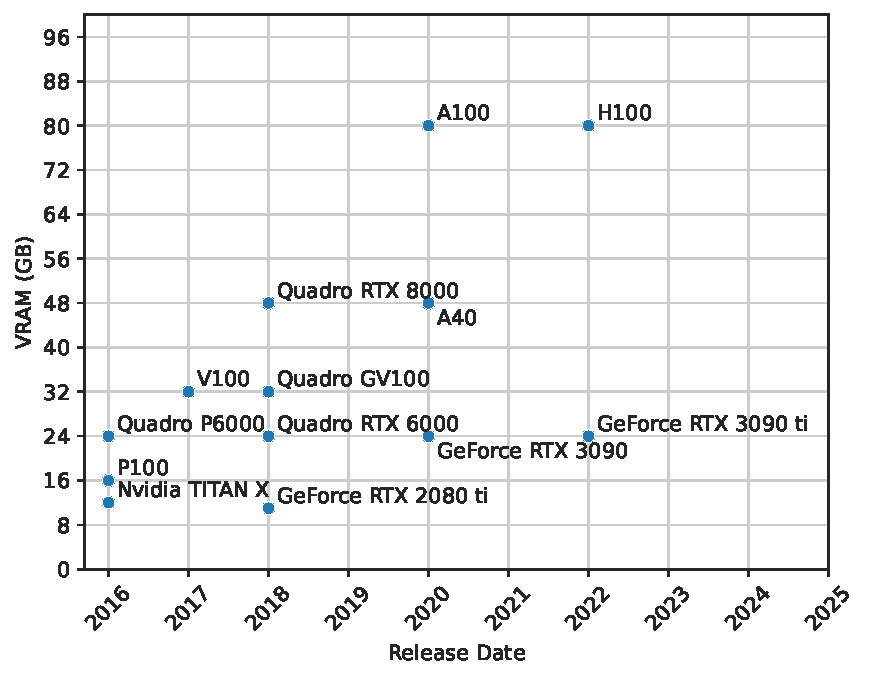
\includegraphics[width=\textwidth]{./figures/gpu-vram-over-time.pdf}
\end{figure}

\begin{figure}[h]
    \caption{Model size over the past 4 years: ELMo \cite{peters2018elmo}, BERT \cite{devlin2018bert}, GPT-2 \cite{radford2019language}, Megatron-LM \cite{shoeybi2019megatronlm}, T-5 \cite{raffael2019t5}, Turing-NLG \cite{microsoft2020turingnlg}, GPT-3 \cite{brown2020gpt3}, Megatron-Turing-NLG \cite{smith2022megatronturingnlg}}
    \label{fig:model-size-over-time}
    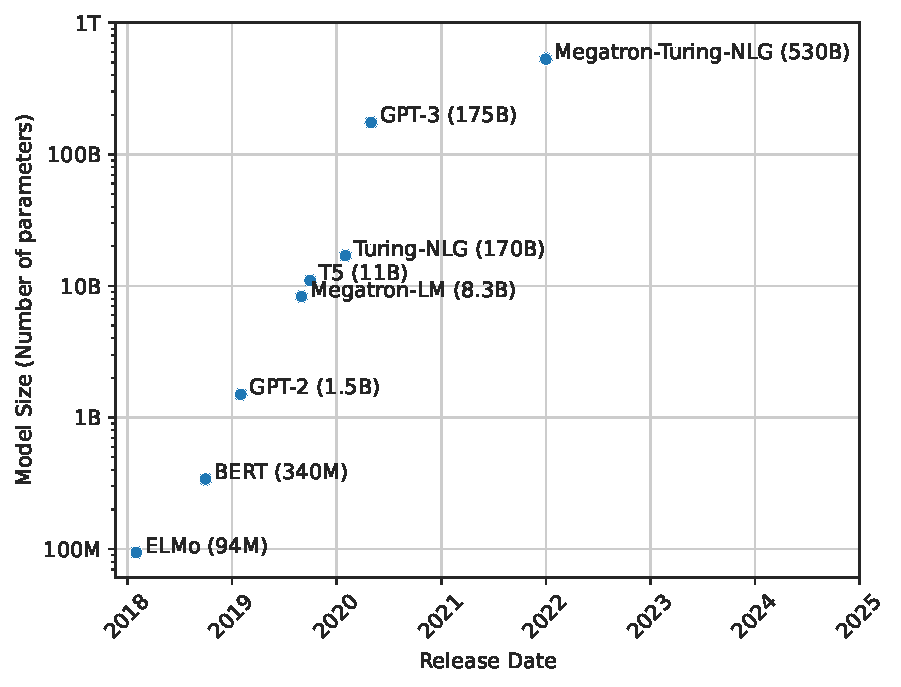
\includegraphics[width=\textwidth]{./figures/model-size-over-time.pdf}
\end{figure}

The characteristics of the latest GPU released by NVIDIA earlier in 2022, the H100 with 80GB of memory, an amount that hasn't changed since its direct predecessor A100.

To tackle this problem, practitioners studied and developed distributed computing techniques to train models that do not fit entirely in a single GPU's memory, distributing the training load to potentially thousands of devices.

These techniques can be briefly categorized as follows:
\begin{itemize}
    \item \textit{Data parallelism}. Given a set of $n$ devices, an instance of the model is trained on each one of the devices. Usually, gradients obtained during backpropagation are then aggregated across all the devices using techniques such as \textit{AllReduce}. This technique however does not work very well with models that exceed a single device's available memory and is therefore used in applications with low-memory devices such as \textit{Federated Learning} \cite{li2019federatedlearning}.

    \item \textit{Model parallelism}. A deep neural network is conceptually split into $n$ partitions across $n$ devices, each hosting a different partition and set of weights. An early notable example of model parallelism is AlexNet \cite{alexnet2012}, where the authors decided to split the computation of some of the layers across two GPUs with 3GB of ram each, a concept illustrated in \autoref{fig:alexnet}. This technique relieves the burden of a single node to host all of the weights of a model but is also more sensitive to issues with communication across nodes.

    \item \textit{Pipeline parallelism}. A combination between model parallelism and data parallelism. Introduced by \cite{huang2018gpipe}, pipeline parallelism consists in splitting a batch into micro-batches across the available computing devices, leading to fewer dead wait times.
    \item \textit{Tensor parallelism}. Tensor operations for huge neural network models can become a bottleneck, as they can require more memory than the host's device can handle and can become slow in general. Tensor parallelism can alleviate a single node's computational burden by splitting a tensor operation across many devices. This technique has been first introduced in neural network models in \cite{dean2012distbelief} with a framework called DistBelief.
    \item \textit{Mixture-of-Experts}. Instead of conceptually splitting a model, we construct multiple, different models. Each of them specializes in a different subset of the complete set of training cases, helped by a gating function. This has been first introduced in 1991 by \cite{Jacobs1991mixtureofexperts} but has recently gained traction due to its attractiveness in numerous tasks.
\end{itemize}

Most of the frameworks and papers built on top of these techniques approach the issues that we have discussed before by employing tremendous amounts of expensive, top-of-the-art and heterogeneous technologies.
However, universities, small companies and hobbyists that want to train the models described in these papers do not necessarily have access to a such vast amount of resources, limiting possibilities and research directions.


Hivemind \cite{riabinin2020hivemind} is a framework that aims to 

\begin{figure}[h]
    \caption{AlexNet \cite{alexnet2012} architecture shows one of the first examples of model parallelism. The training of convolutional layers is split across two GPUs, as the size of the model during training exceeded the available memory of a single GPU.}
    \label{fig:alexnet}
    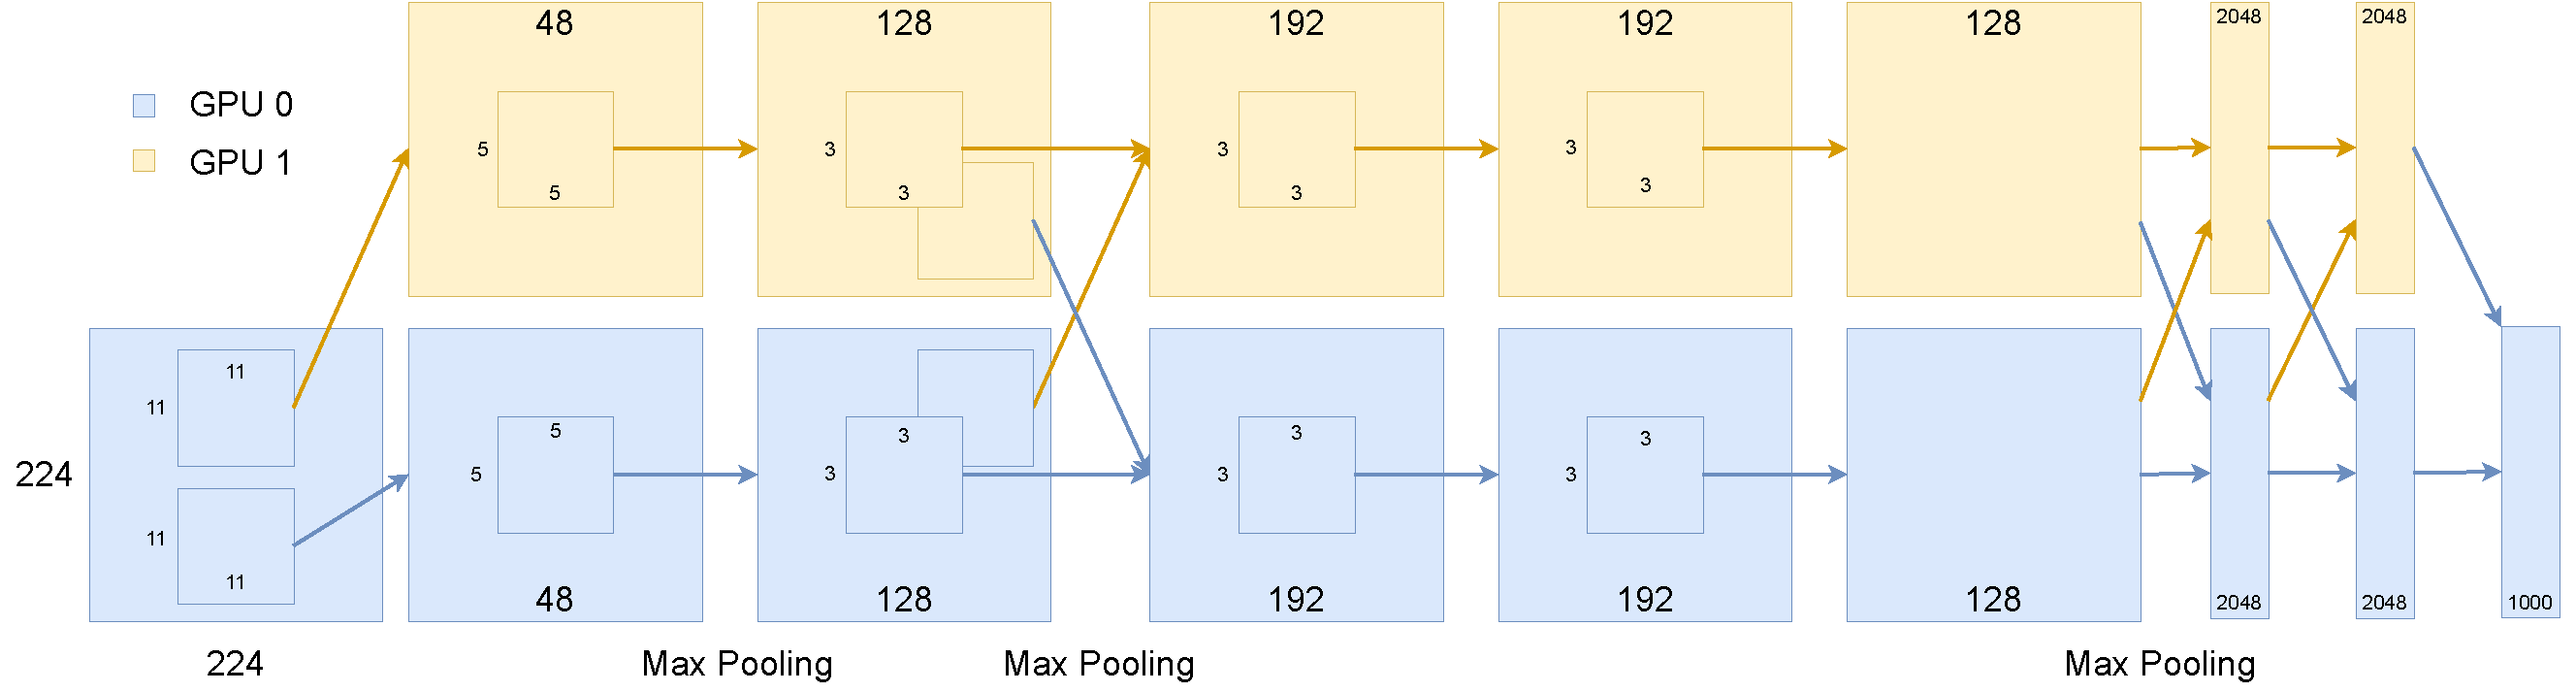
\includegraphics[width=\textwidth]{./figures/alexnet.pdf}
\end{figure}
